% -*- LaTeX -*-
% -*- coding: utf-8 -*-
%
% michael a.g. aïvázis
% california institute of technology
% (c) 1998-2012 all rights reserved
%

\lecture{Introduction to \pyre}{20120518}

% --------------------------------------
% namespace design
\begin{frame}[fragile]
%
  \frametitle{Namespace design}
%
  we are now in a position to assemble the package \package{gauss}; let's start by laying out
  the package namespace
%
  \begin{figure}
    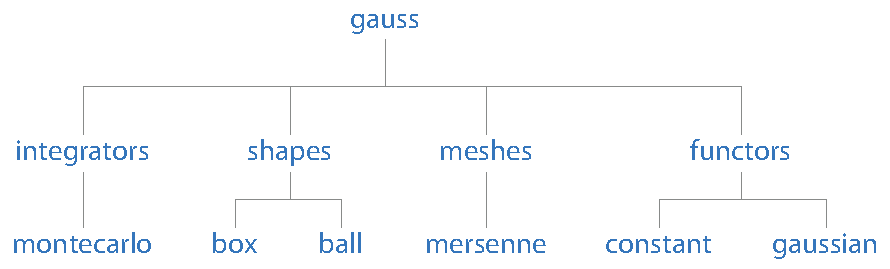
\includegraphics[scale=0.5]{figures/gauss-namespace.pdf}
  \end{figure}
%
  and try to use this layout for both the logical and physical structure
  \begin{itemize}
  \item the top level is our package name
  \item the internal nodes become the names of interfaces and subdirectories
  \item the leaves are the component family names and the names by which the component
    factories are accessible
  \end{itemize}
%
\end{frame}

% --------------------------------------
% shape as a package
\begin{frame}[fragile]
%
  \frametitle{The \package{shapes} package}
%
  in order to make the directory \srcfile{gauss/shapes} as python package, we need to create
  the special file \srcfile{gauss/shapes/\_\_init\_\_.py}
%
  \python{firstnumber=9,linerange={9-14}}{listings/gauss/shapes/__init__.py}
%
  the \keyword{import} statements 
  \begin{itemize}
  \item use \emph{local} imports to make sure that we are accessing the correct modules
  \item create local names for the classes declared inside the named modules
  \end{itemize}
%
  the net effect is to simplify access to the components 
%
  \begin{ipython}{}
    from gauss.shapes import box, ball
  \end{ipython}
\end{frame}

% --------------------------------------
% shapes
\begin{frame}[fragile]
%
  \frametitle{Shapes}
%
  the \interface{Shape} interface in \srcfile{gauss/shapes/Shape.py}
%
  \python{firstnumber=9,linerange={9-37},basicstyle=\tt\tiny}{listings/gauss/shapes/Shape.py}
%
\end{frame}

% --------------------------------------
% balls
\begin{frame}[fragile]
%
  \frametitle{Ball}
%
  the implementation of \component{Ball} in \srcfile{gauss/shapes/Ball.py}
%
  \python{firstnumber=9,linerange={9-42},basicstyle=\tt\tiny}{listings/gauss/shapes/Ball.py}
%
\end{frame}

% --------------------------------------
% balls
\begin{frame}[fragile]
%
  \frametitle{Ball - continued}
%
  \python{firstnumber=43,linerange={43-60}}{listings/gauss/shapes/Ball.py}
%
\end{frame}

% --------------------------------------
% boxes
\begin{frame}[fragile]
%
  \frametitle{Box}
%
  the implementation of \component{Box} in \srcfile{gauss/shapes/Box.py}
%
  \python{firstnumber=9,linerange={9-31}}{listings/gauss/shapes/Box.py}
%
\end{frame}

% --------------------------------------
% boxes
\begin{frame}[fragile]
%
  \frametitle{Box - continued}
%
  \python{firstnumber=32,linerange={32-53}}{listings/gauss/shapes/Box.py}
%
\end{frame}

% end of file 
